\section{Introduction}

\begin{figure*}[!t]
    \centering
    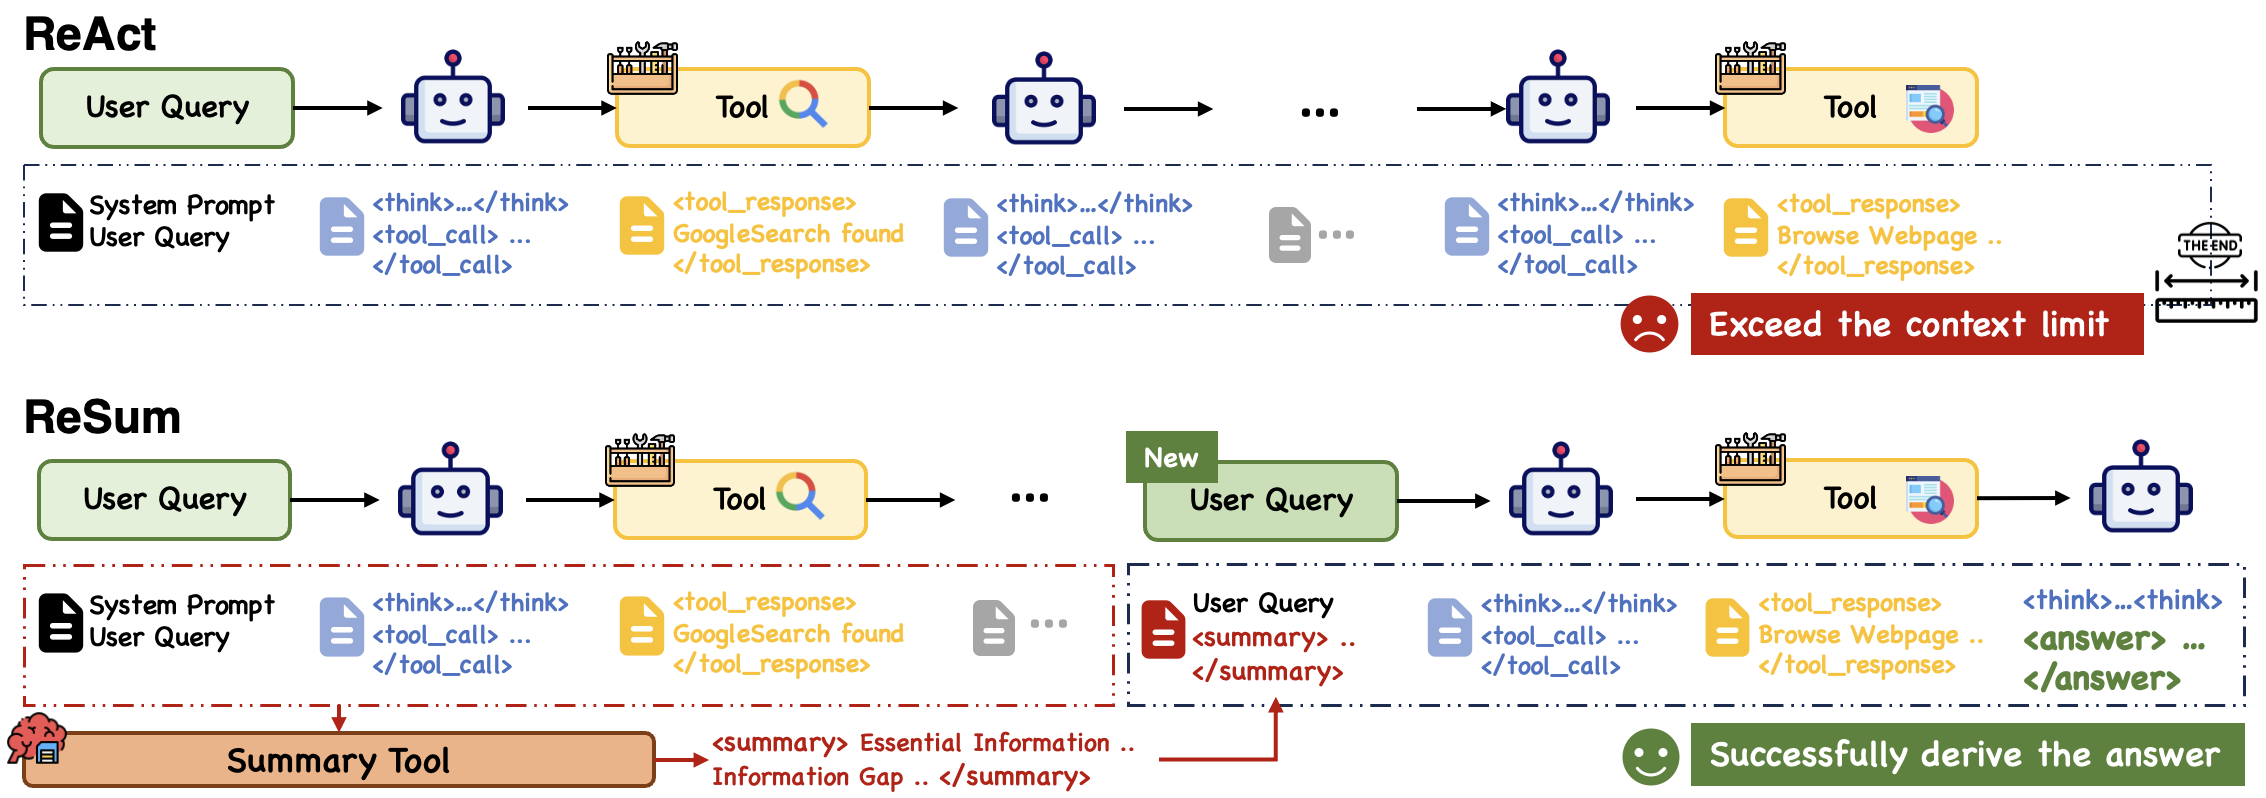
\includegraphics[width=0.95\linewidth]{images/motivation.jpg}
    \caption{\textbf{Comparison between ReAct and ReSum paradigms.} Appending every thought, action, and observation in ReAct exhausts the context budget before multi-turn exploration completes. In contrast, ReSum periodically invokes a summary tool to condense history and resumes reasoning from the compressed summary, enabling indefinite exploration.}
    \label{fig:motivation}
\end{figure*}

Large Language Model (LLM)-based agents have demonstrated strong performance on complex, knowledge-intensive tasks~\citep{yao2023react, wang2024survey, jin2025search, xi2025rise, gao2025asearcher}. Among these, \textbf{web agents} are particularly critical: they actively search and browse the open web, extract and ground facts from diverse sources, and synthesize answers that are both user-specific and up-to-date~\citep{wu2025webdancer, li2025websailor}.

However, answering complex queries is nontrivial. Consider this example: \emph{A painter, whose father died of heart disease, had an elder sister and five children with his wife. Later, his marriage broke down and he had three more relationships. What is the name of the literary work based on this person?} This query exemplifies the challenges of web search: it involves multiple entities, intertwined relationships, and fragmentary information with high uncertainty. Such tasks cannot be resolved with a few simple search calls; instead, they demand extended cycles of targeted querying, browsing, and cross-verification to progressively assemble a complete evidence chain~\citep{gao2025asearcher}.

This need for long-horizon exploration faces a fundamental barrier: context constraints. Most LLMs have limited context windows~\citep{qwen2.5, Jiang2023Mistral7}, and the popular ReAct paradigm~\citep{yao2023react}, which appends every observation and thought to the history, quickly exhausts this budget (\textbf{Figure \ref{fig:motivation}}). Current solutions, such as MEM1~\citep{zhou2025mem1} and MemAgent~\citep{yu2025memagent}, often rely on \textbf{architectural modifications}, e.g., generating internal memory tokens. While effective, these approaches break compatibility with pre-existing agents and necessitate end-to-end retraining.

To overcome these limitations, we introduce \textbf{ReSum}, a lightweight paradigm that enables unbounded exploration through context summarization. The core insight is to \emph{periodically} invoke an external tool to condense interaction histories into compact summaries. By resuming exploration from these compressed states, agents maintain awareness of prior discoveries while freeing up context space. Unlike prior approaches, ReSum represents a \textbf{paradigmatic enhancement} rather than an architectural change, offering a plug-and-play solution that seamlessly empowers an off-the-shelf agent with minimal modifications.
%  with minimal modifications to the standard ReAct loop.

Implementing ReSum effectively requires a powerful summary tool. Generic LLMs often struggle to distinguish key search evidence from noisy, lengthy histories. Therefore, we developed \textbf{ReSumTool-30B} by fine-tuning Qwen3-30B-A3B-Thinking~\citep{qwen3technicalreport} on high-quality $\langle \texttt{Conversation}, \texttt{Summary} \rangle$ pairs derived from powerful open-source models~\citep{r1, gpt-oss}. Building upon a rigorous data construction pipeline, ReSumTool-30B is specifically trained to extract key clues, identify information gaps, and highlight next-step directions, outperforming significantly larger models like DeepSeek-R1-671B~\citep{r1} in summarization quality.

While ReSum is effective in a training-free manner, standard agents can be further optimized to master this paradigm. Therefore, we propose \textbf{ReSum-GRPO}. Unlike supervised fine-tuning, which risks overwriting general capabilities and demands costly expert trajectories, we leverage the self-evolution capabilities of reinforcement learning (RL). This algorithm adapts the classic Group Relative Policy Optimization (GRPO)~\citep{shao2024deepseekmath} to the ReSum paradigm. Specifically, we segment long trajectories at summarization points and employ \textit{advantage broadcasting} to propagate the global advantage derived from final outcome across all segments. This mechanism effectively solves the credit assignment challenge in long-horizon tasks, encouraging agents to both reason effectively from compressed states and collect information that yields high-quality summaries. Our main contributions are summarized as follows:

\begin{itemize}
\item \textbf{ReSum: A plug-and-play paradigm.} We identify the conflict between extensive exploration and context limits. We propose ReSum, a paradigmatic enhancement that periodically compresses history into summaries, enabling indefinite exploration without the architectural modifications required by prior methods.

\item \textbf{ReSumTool-30B: A specialized summary model.} To ensure high-quality summarization in web search contexts, we develop ReSumTool-30B. Through targeted training, it excels at extracting key evidence and guiding future search steps.

\item \textbf{ReSum-GRPO: Paradigm adaptation via RL.} We design ReSum-GRPO to familiarize agents with summary-based reasoning by segmenting long trajectories and broadcasting trajectory-level advantages across all segments. Experiments on three challenging benchmarks show average improvements of 4.5\% for ReSum compared to ReAct, with further improvements of 8.2\% after ReSum-GRPO training.
\end{itemize}

% (其他写法，需要再考虑) This mechanism bridges the credit assignment gap, encouraging agents to reason effectively from compressed states while ensuring early information gathering is properly credited for high-quality summaries.
